% !TEX encoding = UTF-8
% !TEX TS-program = pdflatex
% !TEX root = ../thesis.tex

\chapter{Solution}
Now we discuss the path we decided to take, how we developed the software, 
and the technologies we leveraged. Then, we outline the final achievements 
and what can be done to enhance the PoC potential.
\section{Solution proposal}
After the conducted analysis in the first two weeks, we concluded that building a 
new system from zero would have needed too much time and effort, and especially would 
have required specific advanced skills we did not have.\\
First, we recall that we are building agents for verifiable credentials interaction. 
In a full stack product, our solution is placed between the users, who use secure 
communication protocols\footnote{For example, OAuth or OIDC, as can be seen in the
Figure 3.1},  and VDRs\footnote{For example EBSI, Sovrin or IBSI, blockchain used for
SSI purposes}, which store the DIDs, credentials schema, verification policies, 
and more.
\begin{center}
    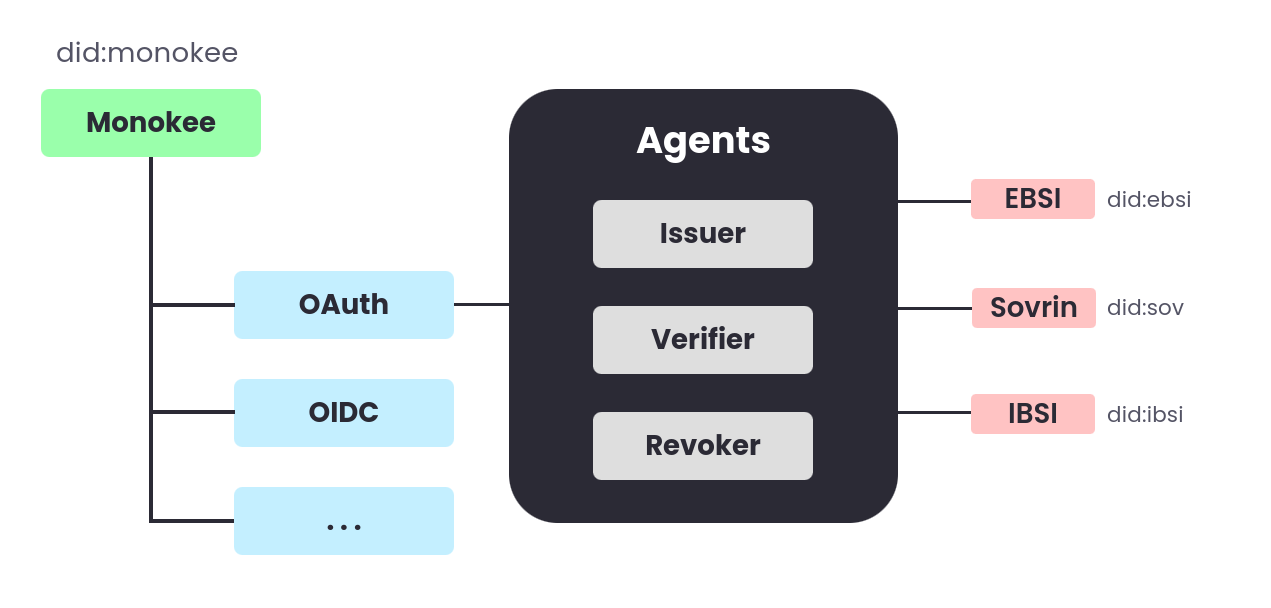
\includegraphics[scale=0.28]{chapter3/problem_schema.png}
    \captionof{figure}{Monokee ideal scenario}
\end{center}
\vspace*{0.5cm}
Figure 3.1 shows the ideal scenario, where Monokee will have its own DID method
(did:monokee), through which will be generated identifiers that will hide (at least,
as far as the user is concerned) the blockchain where it is located.
\vspace*{0.3cm}\\
The final software structure has three main components:
\begin{itemize}
    \item \textbf{Frontend}: it allows the user to interact with the system's core 
    functionalities and serves as an interface for every SSI Kit SDK function.
    \item \textbf{Backend}: it is needed for security, as we will analyze 
    further, and for cryptographic functions that the frontend could not execute.
    \item \textbf{SSI Kit SDK}: it exposes all the SSI functionalities, and enables 
    the user to create keys and DIDs, issue VC, present them as VPs, and more.
    \item \textbf{Smart Contracts}: for what concerns SSI Kit integration, the 
    contracts serve as trusted verifiers and verification results register. Some 
    contracts emit ERC-721 tokens, which let the user request the diploma, but they 
    will not be discussed here.
\end{itemize}
Figure 3.2 shows the system final architecture visualization.
\begin{center}
    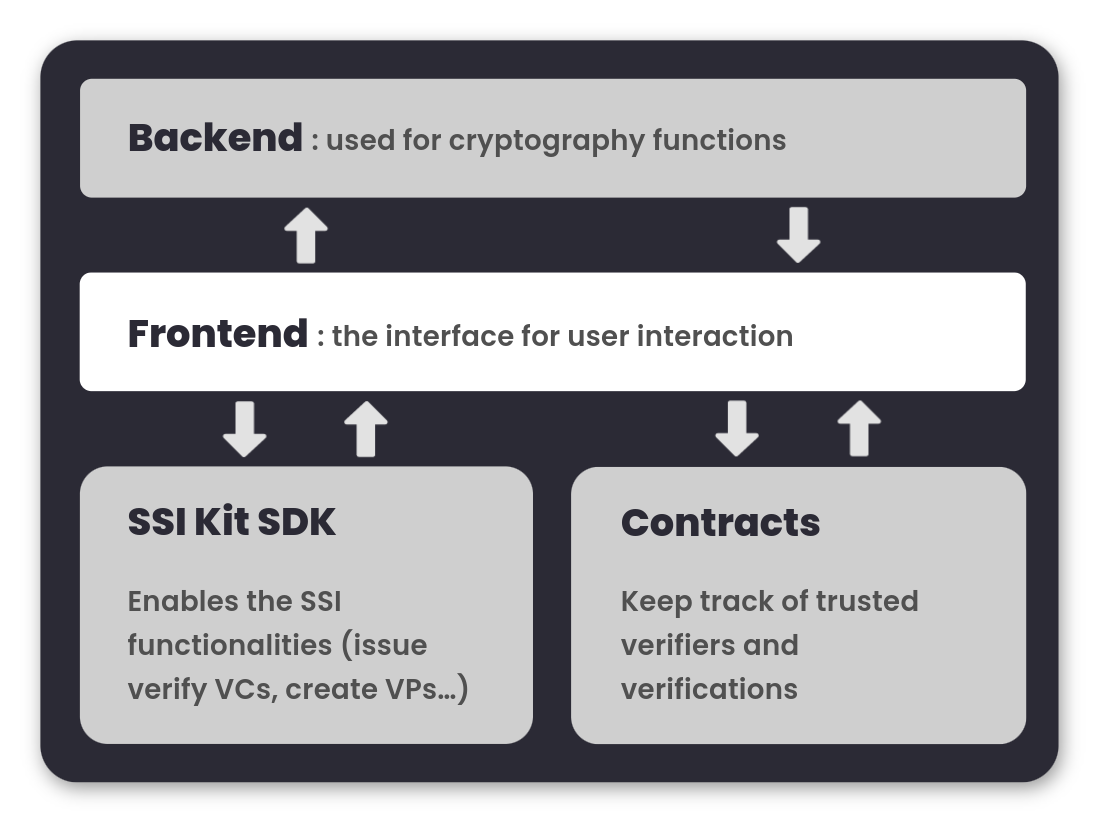
\includegraphics[scale=0.28]{chapter3/structure.png}
    \captionof{figure}{Solution visual representation}
    \label{fig:structure}
\end{center}

\clearpage
\section{Solution development}
In the following sections, we discuss the technologies we used to build the
solution, and we explain the main functionalities of the system.
\subsection{Technologies and Tools}
Before explaining the solution, we list the languages and tools we leveraged to develop it,
for both SSI Kit SDK and PoC.

\subsubsection{Common tools and languages}
\begin{itemize}
    \setlength\itemsep{-0.1em}
    \item \texttt{Typescript}: a strongly typed programming language that builds 
    on JavaScript. It was chosen because the other Monokee's modules were in 
    Typescript, so it would have been easier for the team to integrate. Also, it is 
    very convenient for its strongly typed nature;
    \item \texttt{JSON}: as already covered in \hyperref[subsubsec:json]{Chapter 2}, 
    \texttt{JSON} is a lightweight data-interchange format. It has been extensively used,
    mainly for credentials representation and API calls;
    \item \texttt{Node.js}: a JavaScript runtime built on Chrome's V8 JavaScript
    engine. It has been used for code execution;
    \item \texttt{npm}: a package manager for the JavaScript programming language.
    It has been used to manage the dependencies of the projects;
    \item \texttt{Git}: a free and open-source distributed version control system
    used for tracking and collaboration purposes;
    \item \texttt{Visual Studio Code}: the Integrated Development Environment (IDE)
    we have used for the solution development.
\end{itemize}

\subsubsection[SSI Kit SDK]{SSI Kit SDK\footnote{\texttt{uuid}, \texttt{rfc4648}, 
\texttt{sha256}, and \texttt{nacl} have been used just to generate tokens used for 
credentials revocation, as can be reed \hyperref[method:isRevoked]{here}}}

\begin{itemize}
    \setlength\itemsep{-0.1em}
    \item \texttt{jest}: a JavaScript testing framework. It has been used to test
    the SSI Kit SDK components;
    \item \texttt{waltid-ssikit}: the library written in Kotlin/Java that provides 
    the SSI functionalities set. The developed SDK is a Typescript wrapper of this 
    library;
    \item \texttt{axios}: a promise-based HTTP client for the browser and node.js,
    used to make API calls to waltid-ssikit;
    \item \texttt{uuid}: a library used to generate RFC-compliant Universally Unique
    Identifiers (UUIDs);
    \item \texttt{rfc4648}: a library used to encode and decode data in Base32 format;
    \item \texttt{sha256}: a library used to generate SHA-256 hashes;
    \item \texttt{nacl}: a library used to decode UTF8 \texttt{strings};
\end{itemize}

\subsubsection{Frontend}
\begin{itemize}
    \setlength\itemsep{-0.1em}
    \item \texttt{React.js}: a JavaScript library for building user interfaces. It
    has been used to build the frontend;
    \item \texttt{Chakra-UI}: a simple, modular and accessible components library,
    used with \texttt{React.js} to build the frontend.
    \item \texttt{ethers}: a library used to interact with Ethereum Virtual
    Machine compatible blockchains;
    \item \texttt{wagmi}: a collection of React Hooks containing everything needed
    to start working with Ethereum; it has been used to interact with the smart
    contracts;
    \item \texttt{RainbowKit}: RainbowKit is a React library that makes it easy to 
    add the wallet connection, e.g., for Metamask integration.
    \item \texttt{GraphQL}: the query language used by The Graph;
    \item \texttt{ssikit-sdk}: the developed Typescript SDK used to interact with 
    the SSI Kit library.
    \item \texttt{The Graph}: a decentralized protocol for indexing and querying
    data from blockchains, starting with Ethereum. It makes it possible to query 
    data that is difficult to query directly. It has been used to query The
    deployed smart contracts.
    \item \texttt{smart contracts suite}: a collection of smart contracts used to
    register the verifications and the verification results on-chain.
\end{itemize}

\subsubsection{Backend}
\begin{itemize}
    \setlength\itemsep{-0.1em}
    \item \texttt{Express.js}: a web application framework for Node.js. It has been
    used to build the backend, where the cryptographic functions are executed; the frontend
    calls them through API calls;
    \item \texttt{ssikit-sdk}: the developed Typescript SDK used to interact with
    the SSI Kit library.
    \item \texttt{jose}: a library used to encode and decode \texttt{JSON} Web Tokens (JWTs),
    which have been used to represent private and public keys;
    \item \texttt{nodemon}: a tool that automatically restarts the node application
    when file changes in the directory are detected.
\end{itemize}

\subsection{SSI Kit SDK development}
In this section we describe the SSI Kit SDK development, which is the core of the
solution. The SDK is a Typescript wrapper of the waltid-ssikit library, which is
written in Kotlin/Java. The SDK exposes all the functionalities of the library,
and it is used by the frontend and the backend to interact with the SSI Kit.

\subsubsection{walt.id SSI Kit}
First, we need to know how to interact with it to understand how to build the SDK.
The kit gives us three options:
\begin{itemize}
    \item \textbf{CLI Tool}: it offers a rich set of commands to run the entire functionality 
    the SSI Kit provides. The CLI tool can be used by running the Docker container or
    the executable by the local build.
    \item \textbf{Dependency (JVM)}: it can be used directly as JVM-dependency via Maven or 
    Gradle.
    \item \textbf{REST API}: it can be run as a service, so an application can access its 
    functionalities via REST API.
\end{itemize}
As we decided to build a Typescript SDK, the REST API is the most convenient way 
to access the kit's functionalities: if we chose CLI, every time we call an SDK 
method,  we should have fired a shell command translating the method execution, and 
it would be the most uncomfortable option. The Dependency option, in addition, is 
immediately discardable as we do not use Maven or Gradle (the application is not 
Java/Kotlin based).\\
The REST API service, instead, is very immediate to integrate into an SDK.
In fact, we previously defined the SDK as a "wrapper" because the SDK methods (at 
least, the great majority) forward their execution as an API call to the underlying 
kit. This makes the interaction with the kit a lot easier for Javascript/Typescript 
application based.
\vspace*{0.3cm}\\
Let us now describe how the SSI Kit API is structured to explain later the choices 
made for the SDK development.
\paragraph{Structure.}
The API is divided in five main components:
\begin{itemize}
    \item \textbf{Signatory}: the component that manages the issuing and
    revocation of verifiable credentials. Also, it can list the credential templates
    used to issue them;
    \item \textbf{Custodian}: gives a CRUD interface for keys, DIDs and credentials.
    Here also can be generated VPs;
    \item \textbf{Auditor}: enables the user to manage verification policies,
    and verify any verifiable credential or presentation;
    \item \textbf{ESSIF}: enables the user to interact with EBSI blockchain (e.g.,
    register a DID);
    \item \textbf{Bonus: Core API}: It is a set of functionalities chosen from the 
    above components. However, the team writes in the documentation that it will not 
    be maintained. For this reason we decided to not build a class for this component.
\end{itemize}
Assuming this, we can say it could be a good idea to build a class for each component 
to organize the SDK better and separate the code.

\subsubsection{SSI Kit Typescript SDK}
After analyzing the SSI Kit structure, we can describe how we developed the SDK.
As stated above, we decided to build a class for each SSI Kit component to modularize 
the SDK. In every class, we put a method corresponding to an API call.\\
For API calls, we use Axios, through which we perform a call in each SDK method. So 
a good thing to do is to create a generalized function, called in every method, 
without writing the same code where possible.
\vspace{0.3cm}\\
Figure 3.3 shows a snippet of the \texttt{callAPI} function, which is used to perform
the API calls.
\begin{center}
    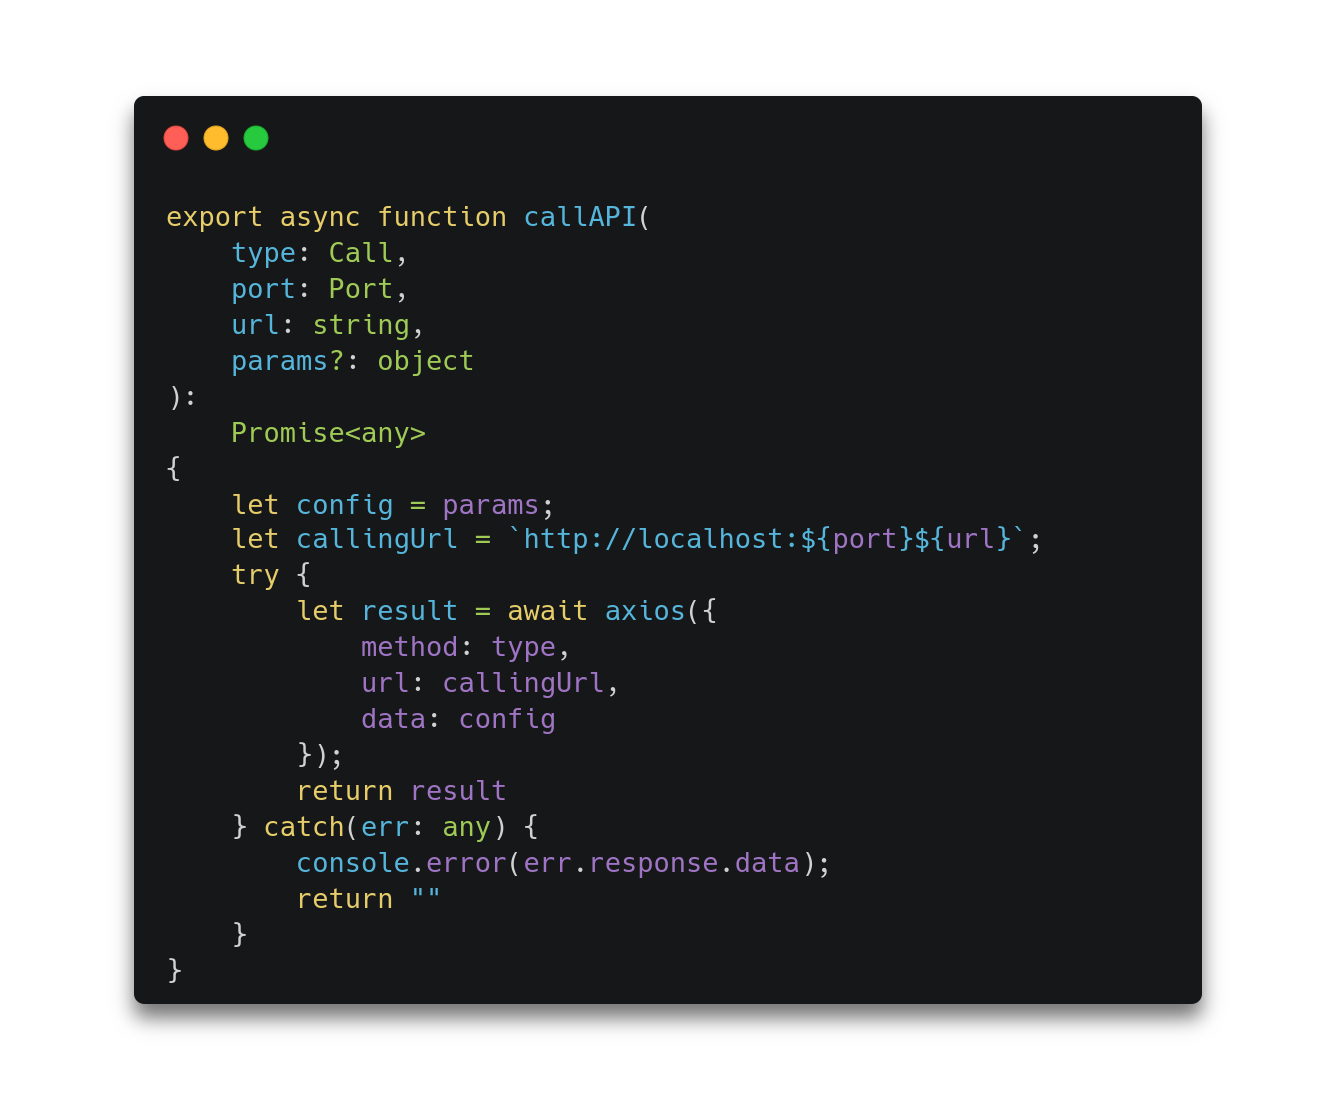
\includegraphics[scale=0.24]{chapter3/callAPIfunction.png}
    \vspace{-0.5cm}
    \captionof{figure}{Snippet of the callAPI function.}
    \label{fig:callAPI}
\end{center}
\vspace{0.5cm}
As input, it takes four parameters:
\begin{itemize}
    \item \texttt{type}: the HTTP method to use; it can be \texttt{"GET"}, \texttt{"POST"},
    \texttt{"PUT"} or \texttt{"DELETE"};
    \item \texttt{port}: the SSI Kit service needs to be run to use the SDK. It then makes
    available four ports, which are used to access the different components of the
    SSI Kit. The \texttt{port} parameter is used to specify which port to use; it can
    be 
    \begin{itemize}
        \item \texttt{7001} (Signatory);
        \item \texttt{7002} (Custodian);
        \item \texttt{7003} (Auditor);
        \item \texttt{7004} (ESSIF);
        \item \texttt{8080} (Universal Resolver);
    \end{itemize}
    \item \texttt{url}: the URL of the API call (e.g., \texttt{"/v1/verify"} to call
    the credentials verification method of the SSI Kit);
    \item \texttt{params}: this is an optional parameter, which is used to pass
    additional info to the call if needed.
\end{itemize}
The return type is generic, as there are many types of results (keys, DIDs, VCs,
booleans, and more). Also, it can be seen that the two parameters \texttt{type} and
\texttt{port} have user defined types. These types and the \texttt{apiCall} function 
can be found inside the file \texttt{utils.ts}, which is a collection of types, 
functions and interfaces used by the SDK, as we analyze in the next section.
\vspace{0.3cm}\\
For the most input/output object parameters of the API calls, we created interfaces
to type them. This is useful to have a better understanding of the parameters, to 
avoid errors and to facilitate the use of the SDK.\\
For verifiable credentials, we did not, as their structure may change from istance
to istance. We simply treat them as \texttt{JSON} objects.\\
We could leave everything as a \texttt{JSON} object, but we decided to create interfaces for
the most important objects. Leaving them as \texttt{JSON} objects would have been a bad idea,
as it would have been difficult to understand what the parameters are and what they
do. The only pro would have been to avoid the creation of interfaces, but we think
that the cons are more important.

\paragraph{Structure.}
The SDK is composed of five main classes. Four are the classes corresponding to the 
four previously described components of the SSI Kit, and the fifth is the one dedicated
to the Universal Resolver. Other than this, the SDK offers a \texttt{utils.ts} file.
\vspace{0.3cm}\\
The SSI Kit SDK splits into three main folders:
\begin{itemize}
    \item \texttt{core}: it contains the main classes of the SDK, which are the
    ones that interact with the SSI Kit API; it also contains the \texttt{utils.ts}
    file, which is a collection of types, functions, and interfaces used by the SDK,
    and the \texttt{lib.ts} file, which contains two functions that perform multiple
    SDK calls (e.g., \texttt{registerDIDOnEBSI} which performs the entire onboarding
    procedure of a DID in the EBSI blockchain);
    \item \texttt{interfaces}: it contains the interfaces used by the four SSI Kit
    class implementations;
    \item \texttt{tests}: it contains the tests of the SDK.
\end{itemize}
Everything (function, type, interface) with the \texttt{export} declaration gets exported by the \texttt{index.ts}
file, which is the entry point of the SDK.

\paragraph{Functionalities.}
After examining the SDK structure, the choices we made, and some technical detail, we can now 
fully explain its functionalities.
\begin{itemize}
    \setlength{\itemsep}{1cm}

    \item \textbf{Signatory}: this class serves as the issuer component in our
    SSI model. It implements five methods:
    \begin{itemize}
        \setlength{\itemsep}{0.4cm}
        \item[] \code{issueCredential}: issues a verifiable credential;
        \begin{itemize}
            \item \textbf{Params}: \texttt{IssueCredentialRequest}, which is an object where 
            it is specified the template ID (chosen by those provided by the SSI Kit), the
            credential data and the proof configuration;
            \item \textbf{Returns}: a W3C Verifiable Credential in \texttt{JSON} format.
        \end{itemize}
        \item[] \code{getVCTemplateIDs}: returns the IDs of all the SDK templates;
        \begin{itemize}
            \item \textbf{Returns}: an \texttt{array} of \texttt{strings}, where each \texttt{string} is a template ID
            (e.g., \texttt{"UniversityDegree"}); these templates are usable in the
            \texttt{issueCredential} method.
        \end{itemize}
        \item[] \code{getVCTemplate}: it returns a specific template;
        \begin{itemize}
            \item \textbf{Params}: the \texttt{templateId} \texttt{string};
            \item \textbf{Returns}: a verifiable credential template in \texttt{JSON} format.
        \end{itemize}
        \item[] \code{isRevoked}: checks if a verifiable credential is revoked;
        \label{method:isRevoked}
        \begin{itemize}
            \item \textbf{Params}: the corresponding \texttt{publicRevocationToken};
            \item \textbf{Returns}: the result of the check, which is an object with the
            fields \texttt{revoked} (boolean) and \texttt{token} (\texttt{string});
            \item \textbf{Notes}: the \texttt{publicRevocationToken} is findable
            inside the \texttt{\seqsplit{credentialStatus}} field of the VC. When an issuer issues
            a VC, the SDK generates a \texttt{private} and a \texttt{public} revocation token. 
            The \texttt{private} has to be saved by the issuer, and can be used to revoke 
            the credential. The \texttt{public} one is included in the VC, and everyone can 
            use it to check if the VC has been revoked or not. Figure 3.4 shows the functions
            used to generate the revocation tokens (in 
            \texttt{utils.ts}). The \texttt{baseToken} is the private one, and is a 
            concatenation of two random UUIDs. The \texttt{publicToken} is the derived by
            the \texttt{baseToken} in this manner: 
            \texttt{base32(sha256(baseToken)).replaceAll("=", "").}
        \end{itemize}
        \begin{center}
            \hspace{-1.5cm}
            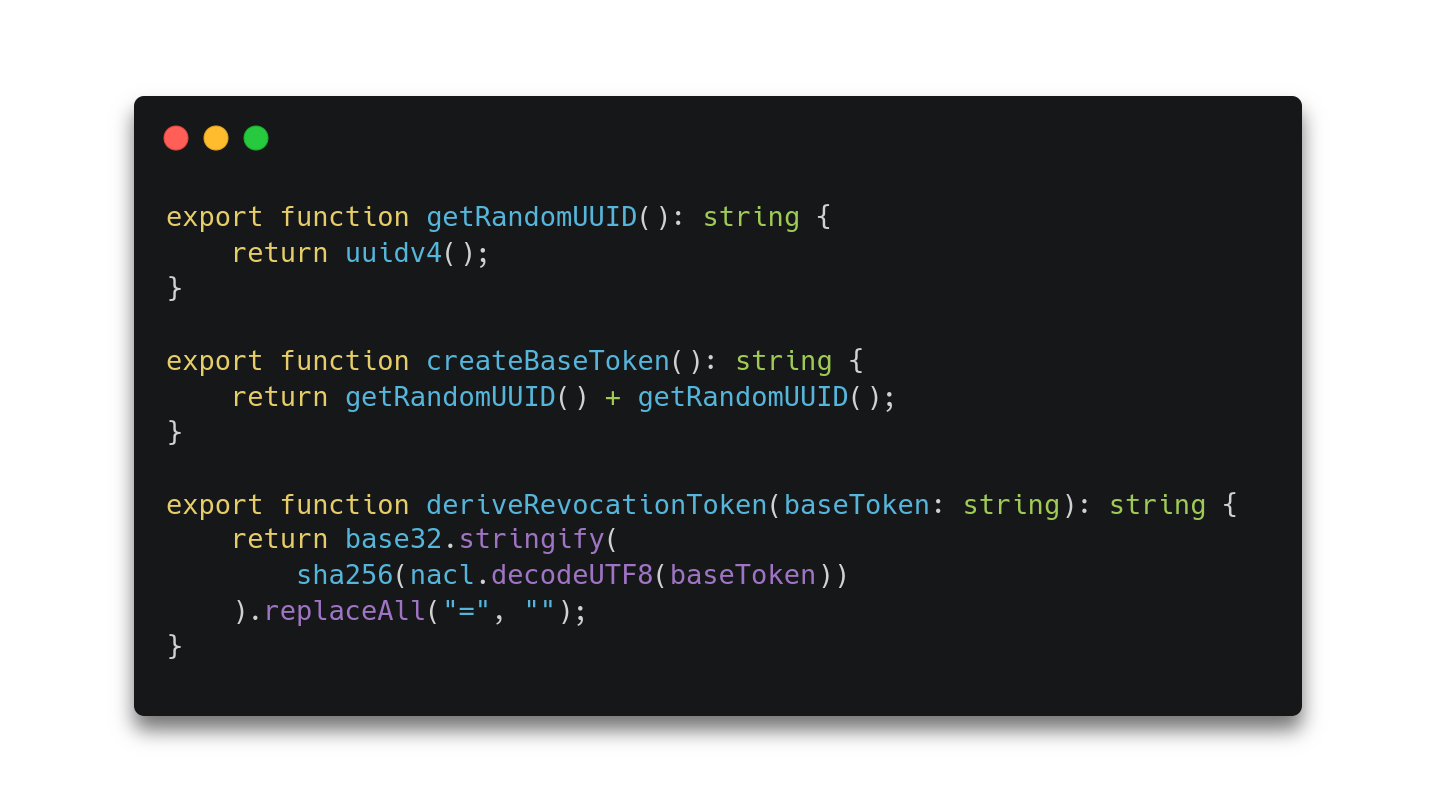
\includegraphics[scale=0.22]{chapter3/revocation.png}
            \vspace{-0.3cm}
            \captionof{figure}{Revocation tokens functions snippet}
        \end{center}
        \vspace{0.3cm}
        \item[] \code{revokeCredential}: revokes a verifiable credential;
        \begin{itemize}
            \item \textbf{Params}: the \texttt{privateRevocationToken}, owned only by the 
            issuer of that VC;
            \item \textbf{Returns}: the revocation result, which is a \texttt{boolean} (if
            \texttt{false}, something went wrong during the process).
        \end{itemize}
    \end{itemize}

    \item \textbf{Custodian}: this class serves as the holder component in our
    SSI model. It implements eighteen methods, and manages keys, DIDs and credentials:
    \begin{itemize}
        \setlength{\itemsep}{0.4cm}
        \item[] \code{getKeys}: gets the keys in the holders's wallet;
        \begin{itemize}
            \item \textbf{Returns}: an \texttt{array} of \texttt{Key} objects, which are the keys
            owned by the holder.
        \end{itemize}
        \item[] \code{getKey}: gets a specific key in the holder's wallet;
        \begin{itemize}
            \item \textbf{Params}: the \texttt{keyId} \texttt{string}, which is the key identifier;
            \item \textbf{Returns}: the corresponding \texttt{Key} object.
        \end{itemize}
        \item[] \code{generateKey}: generates a new key;
        \begin{itemize}
            \item \textbf{Params}: the \texttt{keyAlgorithm} \texttt{string}, that specifies
            the algorithm used to generate the key; the supported algorithms are 
            \texttt{RSA}, \texttt{EdDSA\_Ed25519} and \texttt{EdDSA\_Secp256k1};
            \item \textbf{Returns}: the generated \texttt{Key} object.
        \end{itemize}
        \item[] \code{deleteKey}: deletes a key from the holder's wallet;
        \begin{itemize}
            \item \textbf{Params}: the \texttt{key} parameter, which can be the \texttt{keyId}
            \texttt{string} or the \texttt{Key} object;
            \item \textbf{Returns}: the result of the deletion, which is a \texttt{boolean}.
        \end{itemize}
        \item[] \code{exportKey}: exports a key (private or public) in the desired format;
        \begin{itemize}
            \item \textbf{Params}: the \texttt{key} parameter (\texttt{id string} or \texttt{Key} object),
            the \texttt{format}, which can be \texttt{JWK} or \texttt{PEM}, and \texttt{exportPrivate}
            (if \texttt{true}, the private key is exported, otherwise the public one);
            \item \textbf{Returns}: the exported key in \texttt{JSON} format.
        \end{itemize}
        \item[] \code{importKey}: imports a key in the holder's wallet;
        \begin{itemize}
            \item \textbf{Params}: the \texttt{formattedKey} parameter (\texttt{JWK} or \texttt{PEM} format),
            \item \textbf{Returns}: the \texttt{keyId} of the imported key.
        \end{itemize}
        \item[] \code{getDIDs}: gets the DIDs owned by the holder;
        \begin{itemize}
            \item \textbf{Returns}: an \texttt{array} of \texttt{DID strings}.
        \end{itemize}
        \item[] \code{getDID}: gets a specific DID owned by the holder, from local storage;
        \begin{itemize}
            \item \textbf{Params}: the \texttt{did string};
            \item \textbf{Returns}: the corresponding DID \texttt{JSON} with related metadata
            (e.g., \texttt{verificationMethod}, used to verify the DID signature).
        \end{itemize}
        \item[] \code{createDID}: creates a new DID;
        \begin{itemize}
            \item \textbf{Params}: the \texttt{method} (\texttt{key}, \texttt{web} or \texttt{ebsi}),
            the \texttt{key} (\texttt{object} or id \texttt{string}) used to generate the DID, and
            two optionals (for \texttt{web} method): \texttt{didWebDomain} and \texttt{didWebPath};
            \item \textbf{Returns}: the created DID \texttt{string};
            \item \textbf{Notes}: the DID is in local, so in case of \texttt{ebsi} method
            is needed the \texttt{ESSIF} class to register it on the blockchain.
        \end{itemize}
        \item[] \code{deleteDID}: deletes a DID from the holder's wallet;
        \begin{itemize}
            \item \textbf{Params}: the \texttt{DID} (\texttt{string} or \texttt{object});
            \item \textbf{Returns}: the result of the deletion, which is a \texttt{boolean}.
        \end{itemize}
        \item[] \code{resolveDID}: resolves a DID (in case of \texttt{ebsi} method, it is
        searched on-chain);
        \begin{itemize}
            \item \textbf{Params}: the \texttt{DID string};
            \item \textbf{Returns}: the resolved DID \texttt{JSON} with related metadata.
        \end{itemize}
        \item[] \code{importDID}: resolves and then imports a DID in the holder's wallet;
        \begin{itemize}
            \item \textbf{Params}: the \texttt{DID string};
            \item \textbf{Returns}: the import result, which is a \texttt{boolean}.
        \end{itemize}
        \item[] \code{getCredentials}: gets the credentials owned by the holder;
        \begin{itemize}
            \item \textbf{Returns}: an \texttt{array} of credentials in \texttt{JSON} format.
        \end{itemize}
        \item[] \code{getCredential}: gets a specific credential owned by the holder;
        \begin{itemize}
            \item \textbf{Params}: the \texttt{alias} of the credential (e.g., \texttt{passport});
            \item \textbf{Returns}: the credential in \texttt{JSON} format.
        \end{itemize}
        \item[] \code{getCredentialIDs}: gets the credential IDs (aliases) owned by the holder;
        \begin{itemize}
            \item \textbf{Returns}: an \texttt{array} of credential IDs (\texttt{strings}).
        \end{itemize}
        \item[] \code{storeCredential}: stores a credential in the holder's wallet;
        \begin{itemize}
            \item \textbf{Params}: the the credential's desired \texttt{alias} and the
            \texttt{credential object};
            \item \textbf{Returns}: the storage result, which is a \texttt{boolean}.
        \end{itemize}
        \item[] \code{deleteCredential}: deletes a credential from the holder's wallet;
        \begin{itemize}
            \item \textbf{Params}: the \texttt{alias} of the credential;
            \item \textbf{Returns}: the deletion result, which is a \texttt{boolean}.
        \end{itemize}
        \item[] \code{presentCredentials}: returns the presentation of one or more VCs;
        \begin{itemize}
            \item \textbf{Params}: the \texttt{PresentationRequest} object;
            \item \textbf{Returns}: the \texttt{Presentation} in \texttt{JSON} format;
            \item \textbf{Notes}: the \texttt{PresentationRequest} object is a union of two
            types, \texttt{PresentCredentialsRequest} and \texttt{PresentCredentialIDsRequest};
            in this way, a user can choose to pass the credentials or their IDs; other \texttt{object}
            fields are the \texttt{holderDID}, the \texttt{verifierDID}, and more.
        \end{itemize}
    \end{itemize}

    \item \textbf{Auditor}: this class serves as the verifier component in our
    SSI model. It implements four methods:
    \begin{itemize}
        \setlength{\itemsep}{0.4cm}
        \item[] \code{getVerificationPolicies}: gets the verification policies, usable
        to verify the credentials;
        \begin{itemize}
            \item \textbf{Returns}: an \texttt{array} of \texttt{JSON} objects.
        \end{itemize}
        \item[] \code{verifyCredential}: verifies one or more VCs/VPs;
        \begin{itemize}
            \item \textbf{Params}: the \texttt{VerificationRequest} object, composed by two fields:
            \texttt{credentials} and \texttt{policies};
            \item \textbf{Returns}: the \texttt{VerificationResponse}  object 
            in \texttt{JSON} format (fields: \texttt{valid}, \texttt{results}).
        \end{itemize}
        \item[] \code{createDynamicVerificationPolicy}: creates a verification policy
        usable to verify the credentials;
        \begin{itemize}
            \item \textbf{Params}: the desired \texttt{name}, the \texttt{DynamicPolicyArg} object,
            and two optionals: \texttt{update} (to make it updatable) and 
            \texttt{downloadPolicy} (this depends by \texttt{DynamicPolicyArg});
            \item \textbf{Returns}: the creation result, which is a \texttt{boolean}.
        \end{itemize}
        \item[] \code{deleteDynamicVerificationPolicy}: deletes a verification policy (just
        if it has been created by the user);
        \begin{itemize}
            \item \textbf{Params}: the \texttt{name} of the policy;
            \item \textbf{Returns}: the deletion result, which is a \texttt{boolean}.
        \end{itemize}
    \end{itemize}

    \item \textbf{ESSIF}: it enables the user to interact with EBSI blockchain (e.g.,
    register a DID);
    \begin{itemize}
        \setlength{\itemsep}{0.4cm}
        \item[] \code{onboard}: first step required for a DID registration on EBSI;
        \begin{itemize}
            \item \textbf{Params}: the \texttt{bearerToken}, obtainable from the ebsi
            website, and the \texttt{DID} (\texttt{string} or \texttt{object}) to onboard;
            \item \textbf{Returns}: the VC of the onboarding, or \texttt{false} if the
            onboarding fails.
        \end{itemize}
        \item[] \code{auth}: second step required for a DID registration on EBSI;
        \begin{itemize}
            \item \textbf{Params}: the \texttt{DID} (\texttt{string} or \texttt{object}) to auth;
            \item \textbf{Returns}: the authentication result, which is a \texttt{boolean}.
        \end{itemize}
        \item[] \code{registerDID}: last step required for a DID registration on EBSI;
        \begin{itemize}
            \item \textbf{Params}: the \texttt{DID} (\texttt{string} or \texttt{object}) to register;
            \item \textbf{Returns}: the registration result, which is a \texttt{boolean}.
        \end{itemize}
        \item[] \code{getTimestampByID}: gets the timestamp of a specific transaction;
        \begin{itemize}
            \item \textbf{Params}: the \texttt{transactionID} (\texttt{string});
            \item \textbf{Returns}: the timestamp in \texttt{JSON} format;
            \item \textbf{Notes}: Figure 3.5 shows a timestamp example.
        \end{itemize}
        \clearpage
        \begin{center}
            \label{fig:timestamp}
            \hspace{-1.8cm}
            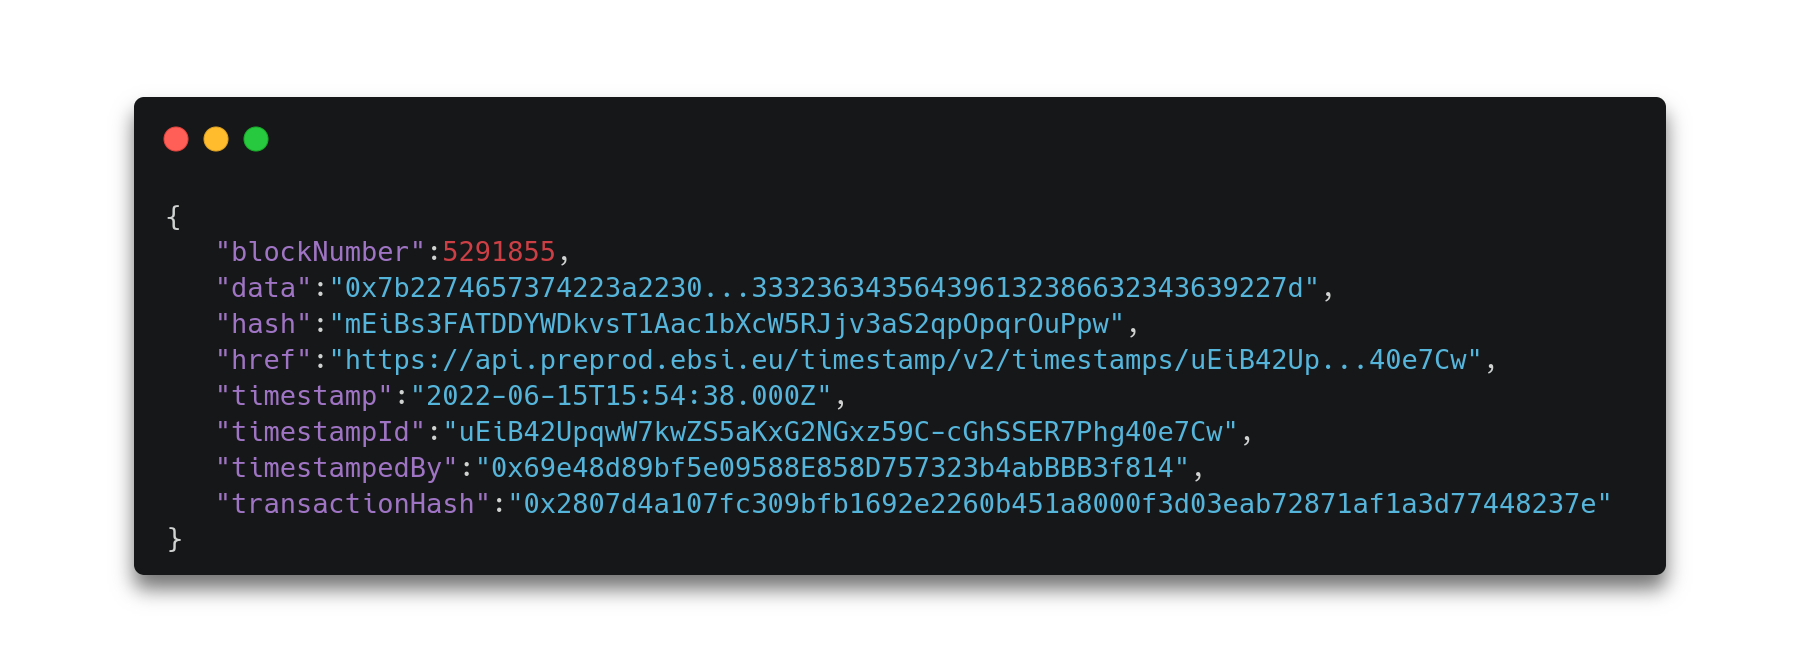
\includegraphics[scale=0.2]{chapter3/timestamp.png}
            \vspace{-0.3cm}
            \captionof{figure}{EBSI transaction timestamp example}
        \end{center}
        \vspace{0.6cm}
        \item[] \code{getTimestampByTXHash}: gets the timestamp of a specific transaction;
        \begin{itemize}
            \item \textbf{Params}: the \texttt{txHash} (\texttt{string});
            \item \textbf{Returns}: the timestamp in \texttt{JSON} format.
        \end{itemize}
    \end{itemize}

    \item \textbf{Universal Resolver}: enables the resolution of DID registered in
    other blockchains than EBSI;
    \begin{itemize}
        \item[] \code{resolveDID}: resolves a DID;
        \begin{itemize}
            \item \textbf{Params}: the \texttt{DID} (\texttt{string});
            \item \textbf{Returns}: the resolved DID in \texttt{JSON} format;
            \item \textbf{Notes}: to see the complete list of supported blockchains,
            refer to the \href{https://github.com/decentralized-identity/universal-resolver}
            {official repository}.
        \end{itemize} 
    \end{itemize}

    \item \textbf{utils.ts}: in these files can be found utilities used in the SDK, but that
    can also be used by the users, such as:
    \begin{itemize}
        \item \textbf{types}, used to enhance the readability of the code, to avoid errors and to
        make the SDK easier to use;
        \item \textbf{consts}, expecially for the API ports;
        \item \textbf{interfaces}, to define the structure of the objects used as input or
        output of the API calls, this way the user can easily understand the structure of
        the objects, and does not need to refer to the documentation each time;
        \item \textbf{functions}, such as \texttt{callAPI} (already \hyperref[fig:callAPI]
        {explained}) or \texttt{getId}, used by the SDK to get the ID of a key or DID.
    \end{itemize}
    
    \item \textbf{lib.ts}: here are placed functions that use multiple SDK methods also from
    different classes. Only two functions have been written so far, and almost only for
    testing purposes, but they can be used by the user as well, and there can be added more 
    in the future if needed.
    
\end{itemize}

\paragraph{Problems and difficulties found.}
The most challenging thing about building the SDK was understanding everything about 
the SSI Kit. The developer needed to learn everything involved in the kit: the W3C 
standards for credentials issuing and verification, the basics of cryptography,  
API interaction, and more.\\
Frequently, the API calls' input or output parameters were not specified in the 
documentation (at least, the schema was specified but not the true meaning of specific
fields). This way, the only manner to go on was to analyze the SSI Kit source code
 (this meant knowing a minimum of Kotlin) or contact the team on Slack.\\
Finally, a minor bug in the Custodian component was found during the SDK development.
It has been reported, and the team fixed it in a week.

\paragraph{Tests.}
The SDK's main components have been tested, focusing on the SSI Kit's four classes 
(Custodian, Signatory, Auditor, and ESSIF).\\
The final coverage is decent but is not 100\%, so it could be slightly improved 
by testing untested branches.t could be slightly improved by testing untested branches.\\
In the underlying images, it can be seen (in this order) all files' final coverage, 
the statements coverage, and finally branches, functions, and lines coverage details.
\vspace{0.5cm}
\begin{center}
    
\includegraphics[scale=0.5]{chapter3/coverage1.png}
    \captionof{figure}{All files' tests coverage percentages}
\end{center}
\begin{center}
    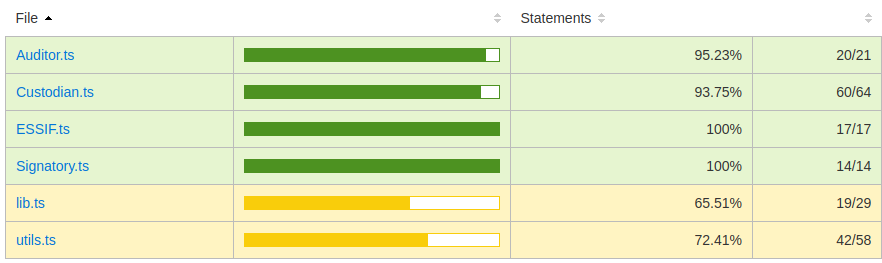
\includegraphics[scale=0.4]{chapter3/coverage2.png}
    \captionof{figure}{Visual representation and statemets coverage}
\end{center}
\begin{center}
    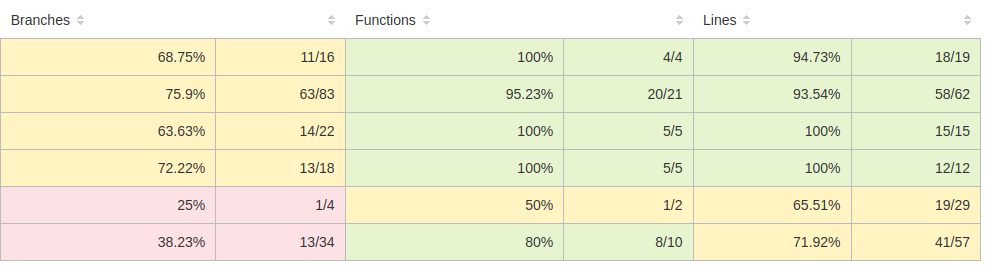
\includegraphics[scale=0.35]{chapter3/coverage3.png}
    \captionof{figure}{Branches, functions, and lines coverage details}
\end{center}

\paragraph{Documentation.}
The SDK documentation can be found at the link
\href{https://matteocasonato.gitbook.io/ssikit-sdk/}
{\seqsplit{https://matteocasonato.gitbook.io/ssikit-sdk/}}. Here can be seen the 
specifications of the SDK classes and methods and some use examples.

\subsection{Web Application Proof of Concept}
After the SDK and smart contracts development, we merged the two macro components 
into a basic web application as a proof of concept of the final solution.\\
The application serves as an interface for smart contract and SDK interaction, 
enabling users to interact with verifiable credentials.

\subsubsection{Structure}
The whole application can be divided into two main components: the frontend, which
contains the central part of the logic, thanks to React.js, and the backend, used 
just because some operations would not have been secure if done in the frontend, and 
something could not be done here because of compatibility issues (browser do not 
support all the cryptographic functions, as we explain later).

\paragraph{Frontend.}
The frontend breaks down into six main pages:
\begin{itemize}
    \item \textbf{Holder}: provides a complete interface for the SDK \texttt{Custodian}
    class; this component is divided into three sub-components:
    \begin{itemize}
        \item[] \textbf{Keys}: here the user can manage the keys used to generate
        the DIDs. The user can create a new key, export it, delete it and more;
        \item[] \textbf{DIDs}: here the user can manage their DIDs. The user can create
        a new DID, load it, delete it;
        \item[] \textbf{Credentials}: here the user can manage their credentials. The
        user can import a new credential, present it and delete it.
    \end{itemize}
    \item \textbf{Issuer}: provides a complete interface for the SDK \texttt{Signatory}
    class; this component is divided into two sub-components:
    \begin{itemize}
        \item[] \textbf{Issue}: in this component, the user can issue a credential.
        \item[] \textbf{Revocations}: in this component, the user can revoke a credential
        or check if a credential is revoked.
    \end{itemize}
    \item \textbf{Verifier}: provides a complete interface for the SDK \texttt{Auditor}
    class, and adds the on-chain functionalities for the verifiers; it is divided into 
    two sub-components:
    \begin{itemize}
        \item[] \textbf{Verifications}: here is possible to verify credentials and put the
        result on-chain as a verification record; also, verification records are searchable;
        \item[] \textbf{Verifiers}: here the smart contracts owner can add new verifiers
        and search them on-chain;
    \end{itemize}
    \item \textbf{Contracts}: on this page, the smart contracts owner can register a new
    contract as trusted or untrusted, and search them on-chain;
    \item \textbf{Diploma}: on this page, an hypothetical student can request a diploma request
    NFT, and then consume it to gain access to the final diploma certificate (VC);
    \item \textbf{EBSI}: here an user can register a DID (generated with \texttt(ebsi)
    method) on the EBSI network; serves as an interface for the SDK \texttt{ESSIF} class.
\end{itemize}
Finally, the application provides the user a web3 wallet connector, so he can interact
with the smart contracts where needed.

\paragraph{Backend.}
We needed to add a backend to our application for two important reasons:
\begin{enumerate}
    \item \textbf{Security}: the frontend is not secure enough to handle cryptographic
    operations, so we needed to move them to the backend; Specifically, when a 
    verifier wants to add a new verification record, he must create a signature with 
    the private key of its DID. The signature certificates that the real verifier is
    adding that record. As the application must interact with the user's private key, 
    this must be done at the backend level: if the private key reaches the frontend, 
    it is no longer secure. We avoided this by using the server as a REST API: when 
    it has to sign, the user passes its private key's (public) ID. The backend creates
    the signature, and it is passed to the frontend. The signature can also be 
    verified with another method.
    \item \textbf{Compatibility}: the browser does not support all the cryptographic
    functions we need. In particular, we needed the elliptic curve Secp256k1, used 
    for Ethereum accounts generation. The DID generated with the ebsi method must be 
    created with a Secp256k1 key pair because when there is an interaction with the 
    blockchain, the EBSI API will sign a message using the corresponding private key
    (which has to be compatible with an Ethereum account).\\
    Assuming this, if we use cryptographic functions from the frontend (using 
    React.js), the application will interact with the W3C Web Cryptography API. 
    Unfortunately, this API does not support the Secp256k1 curve, so we have been 
    forced to move this logic to the backend. 
\end{enumerate}

\subsubsection{Functionalities}
We now examine what the two main components of the web application, frontend, and 
backend, offer (obviously, the frontend offers functionalities to users, and the 
backend serves only the frontend).
\paragraph{Frontend.}
Now we show all the functionalities provided by each previously explained frontend's 
page.
\subparagraph{Holder.} This page is divided into three sections: \texttt{Keys}, 
\texttt{DIDs} and \texttt{Credentials}; Figure 3.9 shows the page screenshot.
\begin{center}
    \begin{tcolorbox}[
        beamer,
        width=0.6\textheight,
        arc=0pt,
        boxsep=0pt,
        left=0pt,right=0pt,top=0pt,bottom=0pt,
        ]
    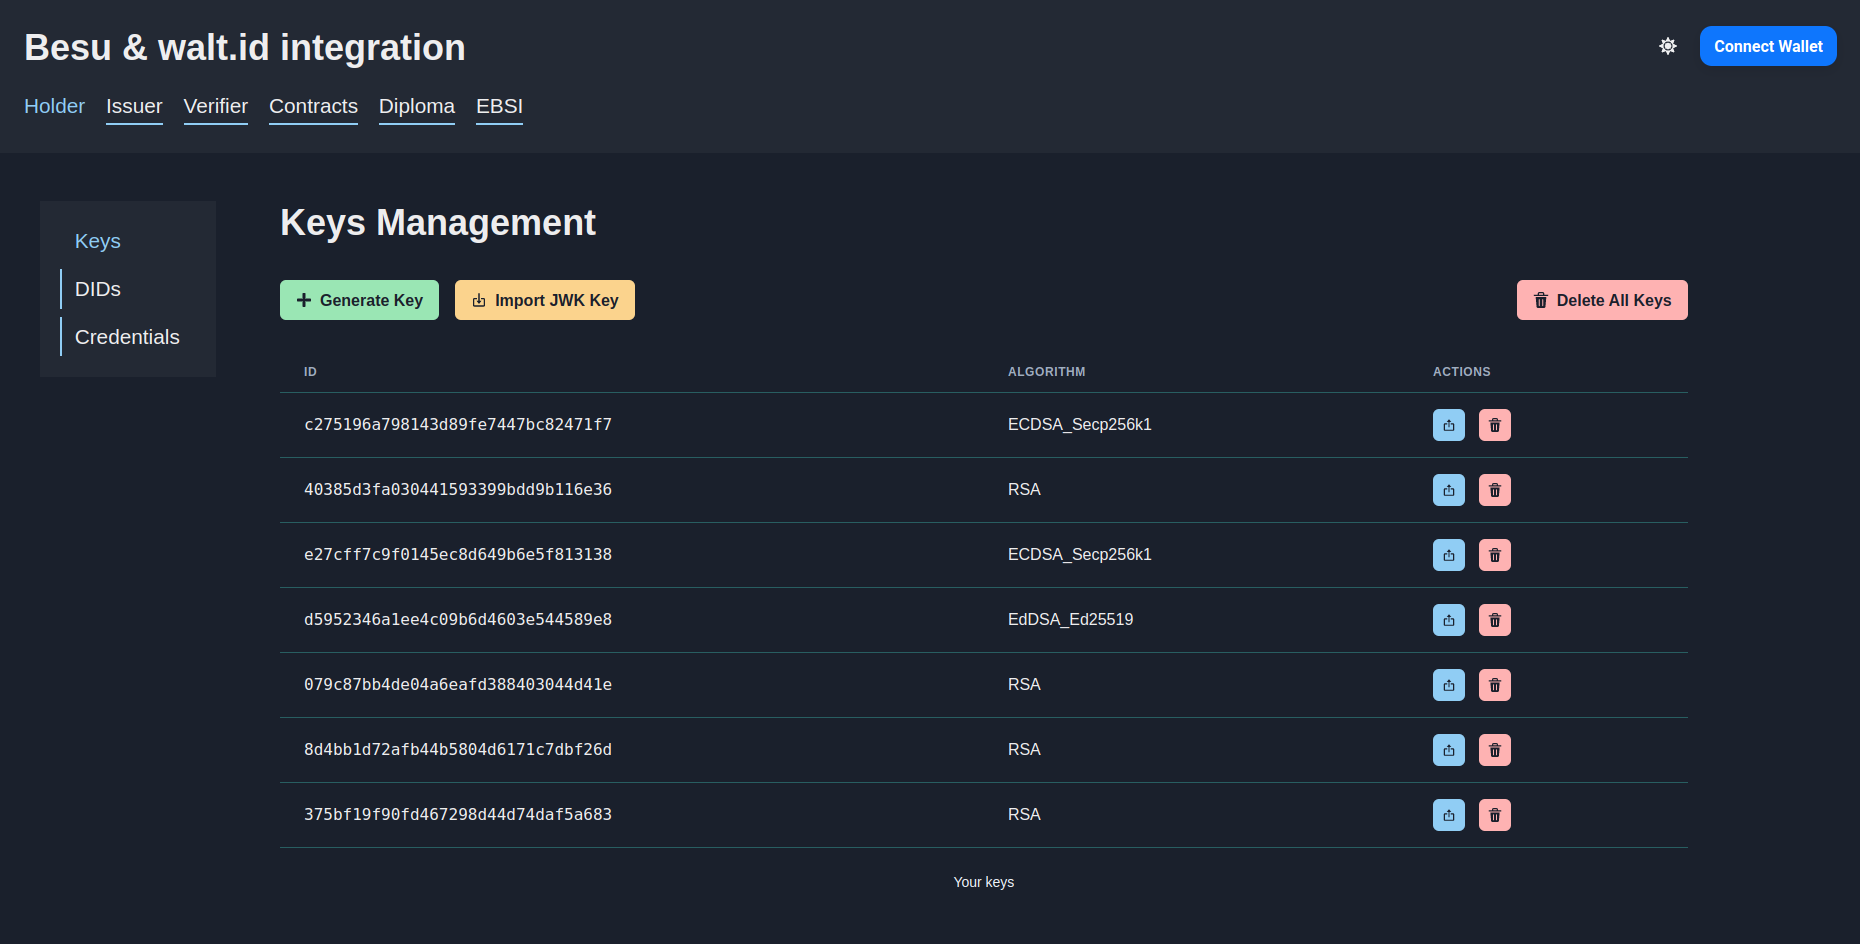
\includegraphics[width=\linewidth]{chapter3/frontend/holder.png}
    \end{tcolorbox}
    \vspace{-0.3cm}
    \captionof{figure}{The \texttt{Holder} page (\texttt{Keys} section)}
\end{center}
In the \texttt{Keys} section inside the \texttt{Holder} page, a user can:
\begin{itemize}
    \item Generate a key using a supported algorithm, by pressing the green button \texttt{Generate Key};
    \item Import a key in \texttt{JWK} format, yellow button;
    \item Export a key (public or private) in the desired format, by pressing the
    blue button;
    \item Delete a key, by pressing the red button;
    \item Delete all the keys, by pressing the red button \texttt{Delete All Keys};
\end{itemize}
\vspace*{0.3cm}
In the \texttt{DIDs} section, a user can:
\begin{itemize}
    \item Create a DID using a supported method and a previously generated key, 
    by pressing the button \texttt{Create DID};
    \item Import a DID inserting its string, by pressing the button \texttt{Import DID};
    \item Resolve a DID by pressing the button \texttt{Resolve DID} (remembering that
    \texttt{did:key} are in local, and \texttt{did:ebsi} are resolved from the blockchain);
    \item View a DID loading it from the local storage by pressing the button in the table;
    \item Delete a DID (from local storage) by pressing the button in the table;
    \item Delete all the DIDs, by pressing the button \texttt{Delete All DIDs};
\end{itemize}
\vspace*{0.3cm}
In the \texttt{Credentials} section, a user can:
\begin{itemize}
    \item Import a credential, giving it an alias, by pressing the button \texttt{Import Credential};
    \item Present one or more credentials, selecting them in the credentials table
    and by pressing the button \texttt{Present Credential};
    \item View a credential loading it from the local storage by pressing the button in the table;
    \item Delete a credential by pressing the button in the table;
    \item Delete all the credentials, by pressing the button \texttt{Delete All Credentials};
\end{itemize}

\clearpage
\subparagraph{Issuer.} This page is divided into two sections: \texttt{Issue}
and \texttt{Revocations}; Figure 3.10 shows the page screenshot.
\begin{center}
    \begin{tcolorbox}[
        beamer,
        width=0.6\textheight,
        arc=0pt,
        boxsep=0pt,
        left=0pt,right=0pt,top=0pt,bottom=0pt,
        ]
    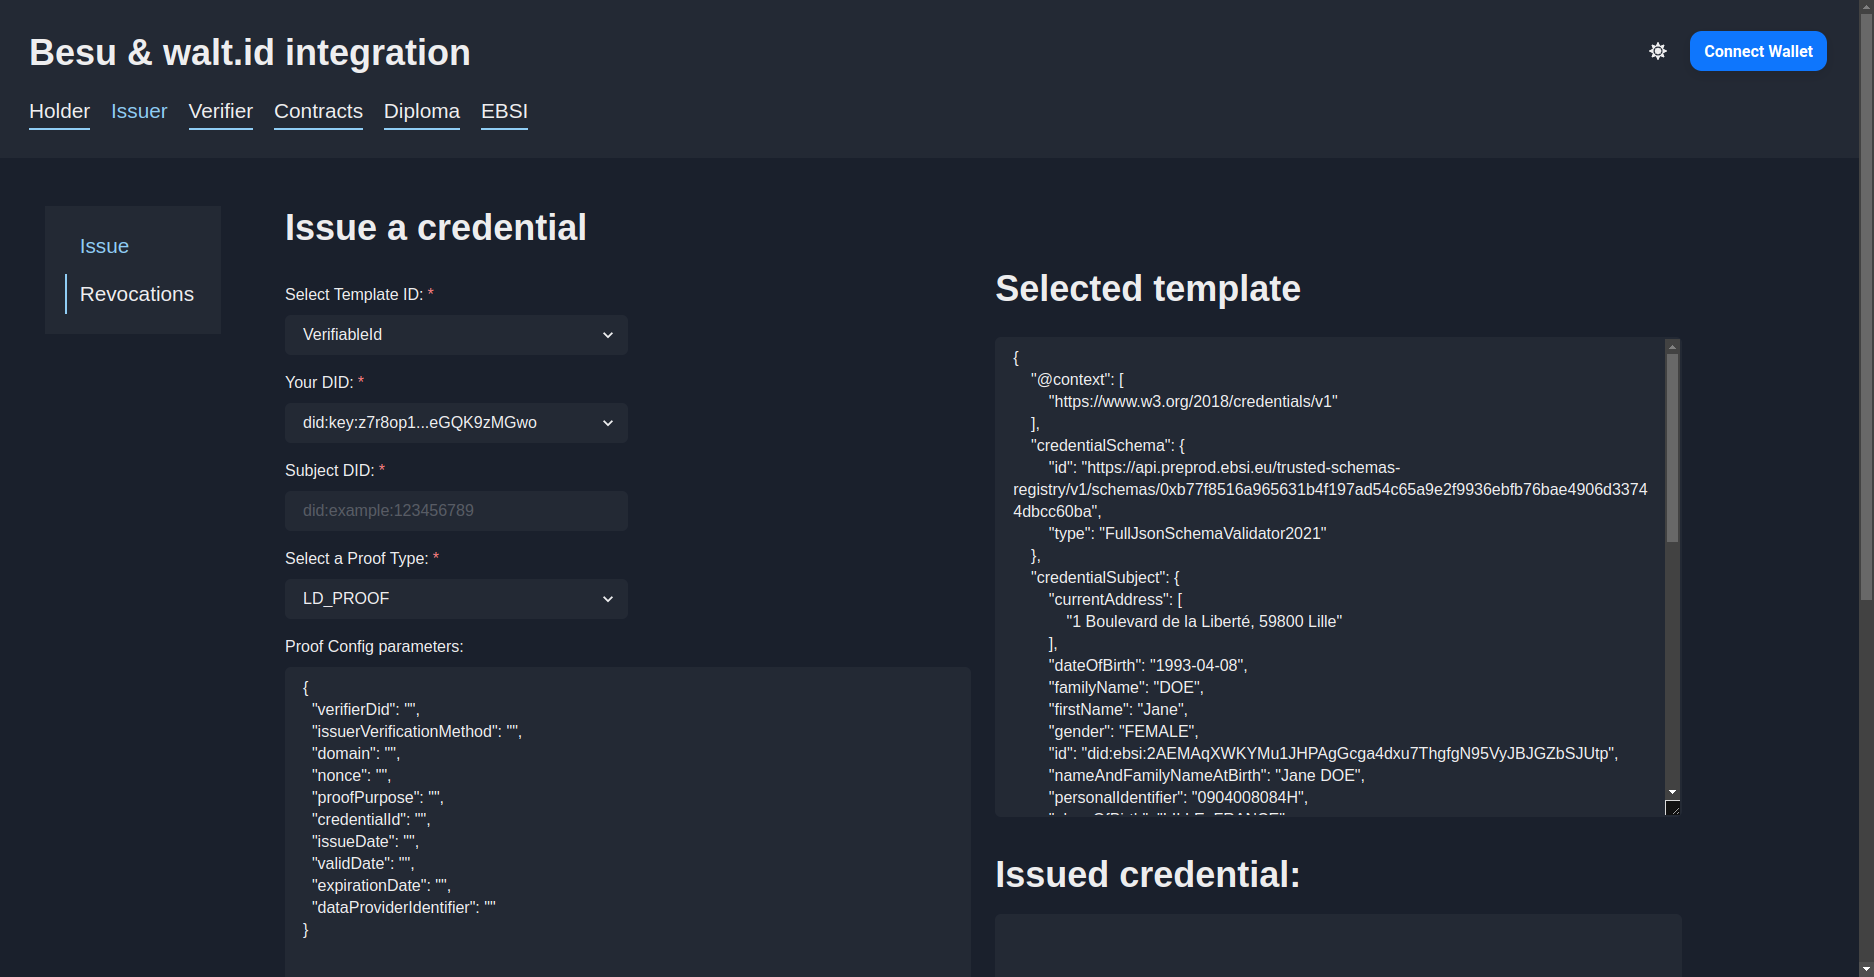
\includegraphics[width=\linewidth]{chapter3/frontend/issuer.png}
    \end{tcolorbox}
    \captionof{figure}{The \texttt{Issuer} page (\texttt{Issue} section)}
\end{center}
In the \texttt{Issue} section, an issuer can issue a credential by filling out the form and
by pressing the button \texttt{Issue Credential}. First, he must select a template,
used for the generation. Then, he must configure the credential, with the possibility
of adding optional fields. The credential is then generated
and inserted in the \texttt{Issued credential} field, and we can copy that and import
locally the issued VC in the \texttt{Holder} page. In a real use case, the credential
would be sent to the holder using secure communication protocols such as \texttt{OIDC}.
\vspace*{0.3cm}\\
In the \texttt{Revocations} section, an issuer can revoke a credential by inserting
the corresponding private revocation token he generated when he issued the credential.
The revocation is off-chain, and we have not yet implemented the on-chain call (from the
frontend) that would change the verification record (however, the function is
implemented in the smart contract). Also, anyone can check if the credential has been
revoked by inserting the corresponding public revocation token.

\clearpage
\subparagraph{Verifier.} This page is divided into two sections: \texttt{Verifications}
and \texttt{Verifiers}; Figure 3.11 shows the page screenshot.
\begin{center}
    \begin{tcolorbox}[
        beamer,
        width=0.6\textheight,
        arc=0pt,
        boxsep=0pt,
        left=0pt,right=0pt,top=0pt,bottom=0pt,
        ]
    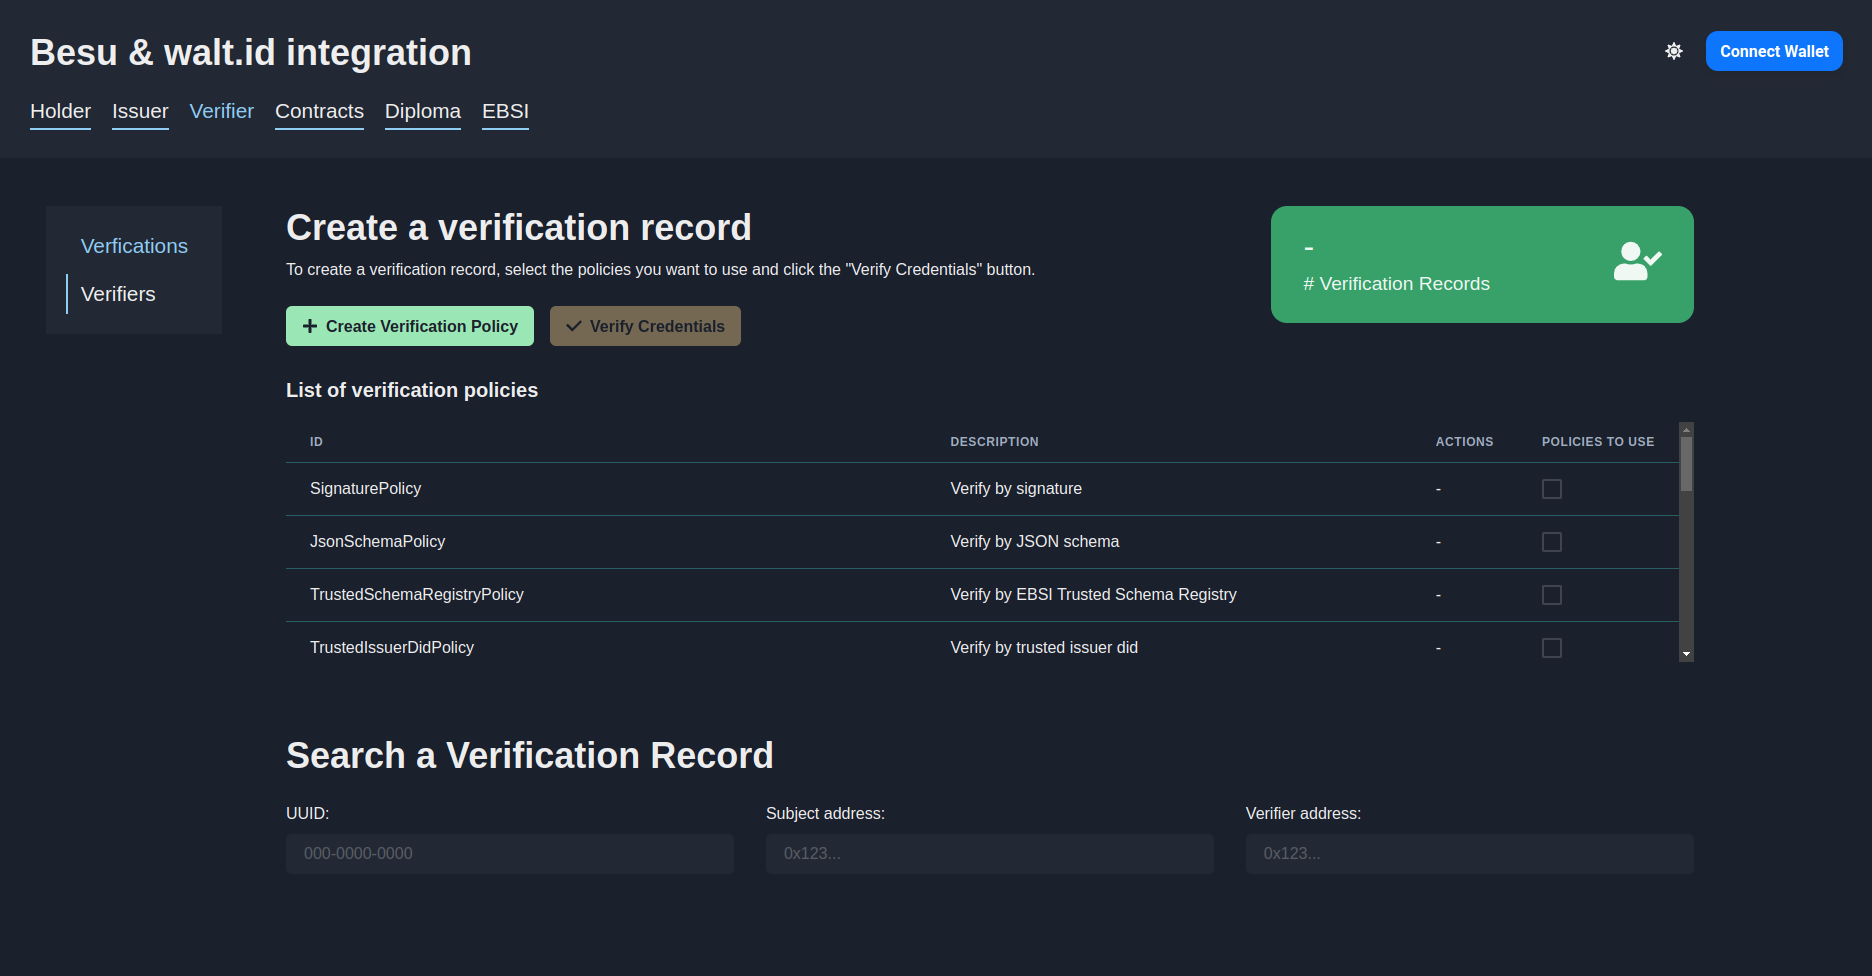
\includegraphics[width=\linewidth]{chapter3/frontend/verifier.png}
    \end{tcolorbox}
    \captionof{figure}{The \texttt{Verifier} page (\texttt{Verifications} section)}
\end{center}
\vspace{0.3cm}
In the \texttt{Verifications} section, a verifier can:
\begin{itemize}
    \item Create a verification policy by pressing the green button;
    \item Verify a credential and register the result on-chain as a verification record. 
    To do so, he must select at least a verification policy from the list.
    Before adding the result on-chain, the verifier creates a signature with the 
    private key of its DID. This way, anyone can resolve their DID and use the public 
    key (findable in the credential's \texttt{verificationMethod} field) to verify the 
    signature;
    \item Search for an on-chain verification record.
\end{itemize}
\vspace*{0.3cm}
In the \texttt{Verifiers} section, the contract owner can register on-chain a new 
verifier, adding it to the trusted verifiers' list. Anyone here can see the list of
trusted verifiers and search for a specific one.
Here is where we manage to merge the off-chain and on-chain solutions in
the PoC. Other functionalities can be added (e.g., on-chain revocation after off-chain
happened), but for time reasons, we have only implemented the verification record 
registration.

\clearpage
\subparagraph{Contracts.} Figure 3.12 shows the page screenshot.
\begin{center}
    \begin{tcolorbox}[
        beamer,
        width=0.6\textheight,
        arc=0pt,
        boxsep=0pt,
        left=0pt,right=0pt,top=0pt,bottom=0pt,
        ]
    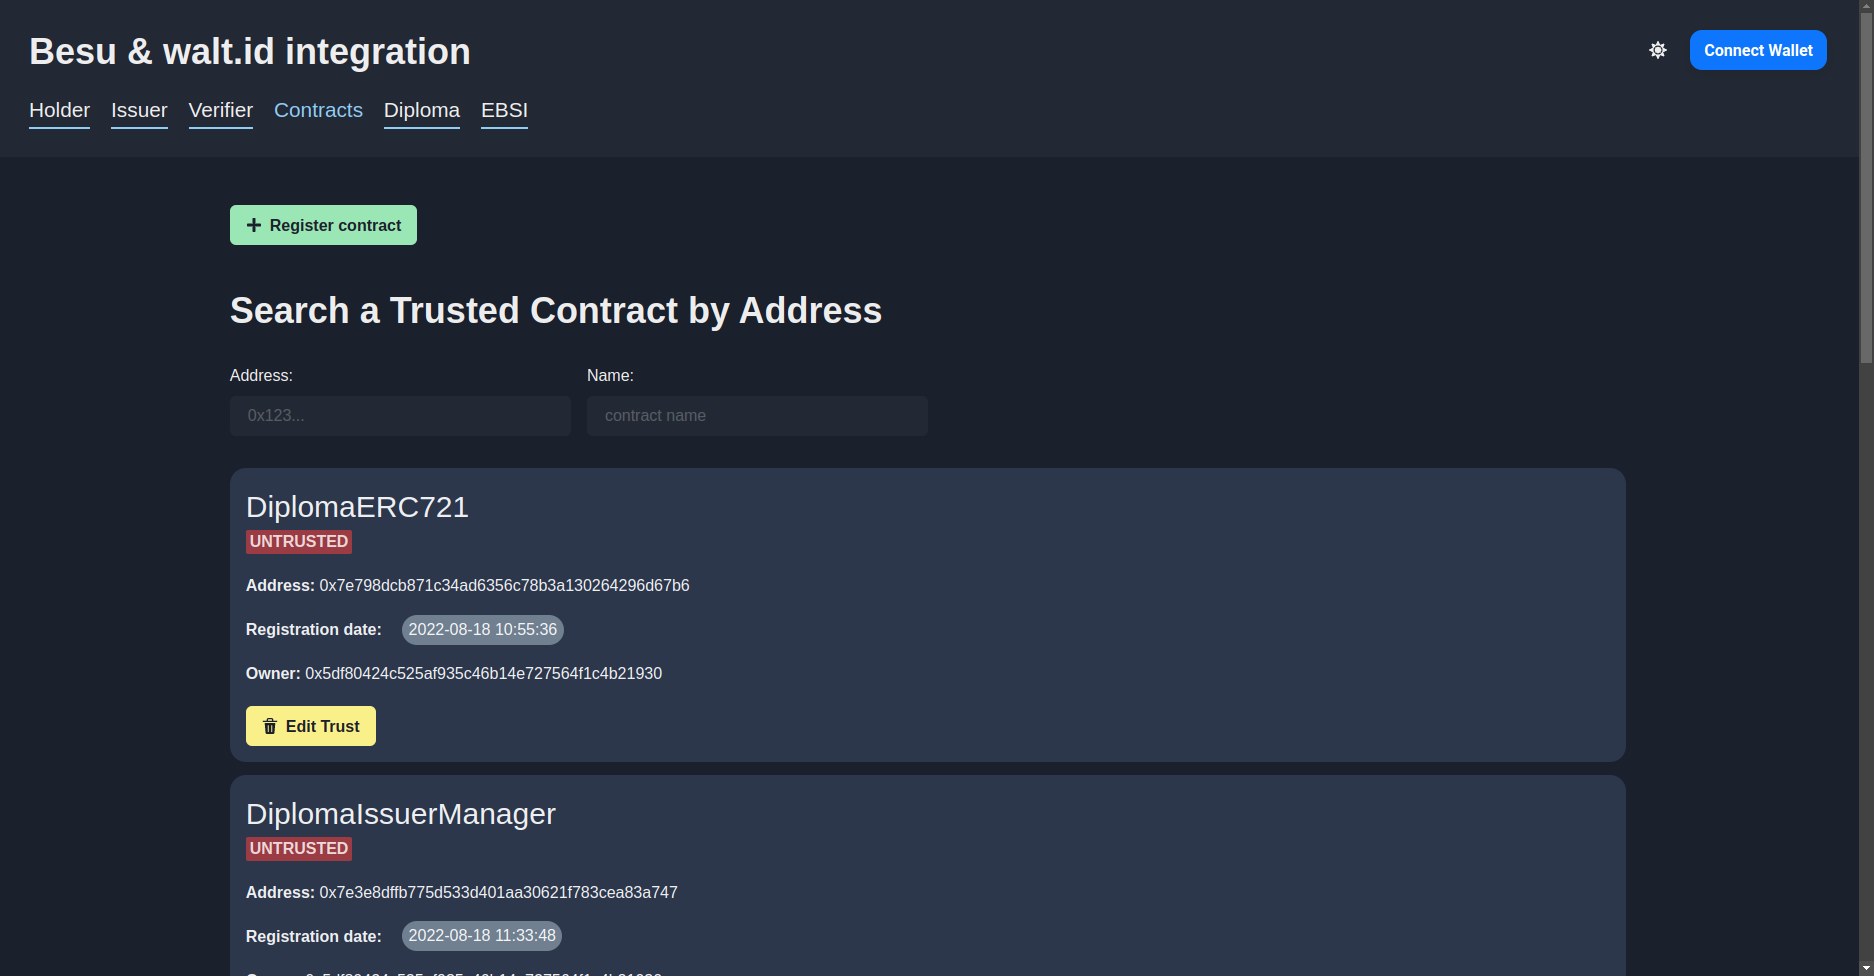
\includegraphics[width=\linewidth]{chapter3/frontend/contracts.png}
    \end{tcolorbox}
    \captionof{figure}{The \texttt{Contracts} page}
\end{center}
On this page, the contract owner can register a contract as trusted or untrusted
in the on-chain list. Anyone can see the list of contracts and search for
a specific one.

\vspace{1cm}
\subparagraph{Diploma.} Figure 3.13 shows the page screenshot.
\begin{center}
    \begin{tcolorbox}[
        beamer,
        width=0.6\textheight,
        arc=0pt,
        boxsep=0pt,
        left=0pt,right=0pt,top=0pt,bottom=0pt,
        ]
    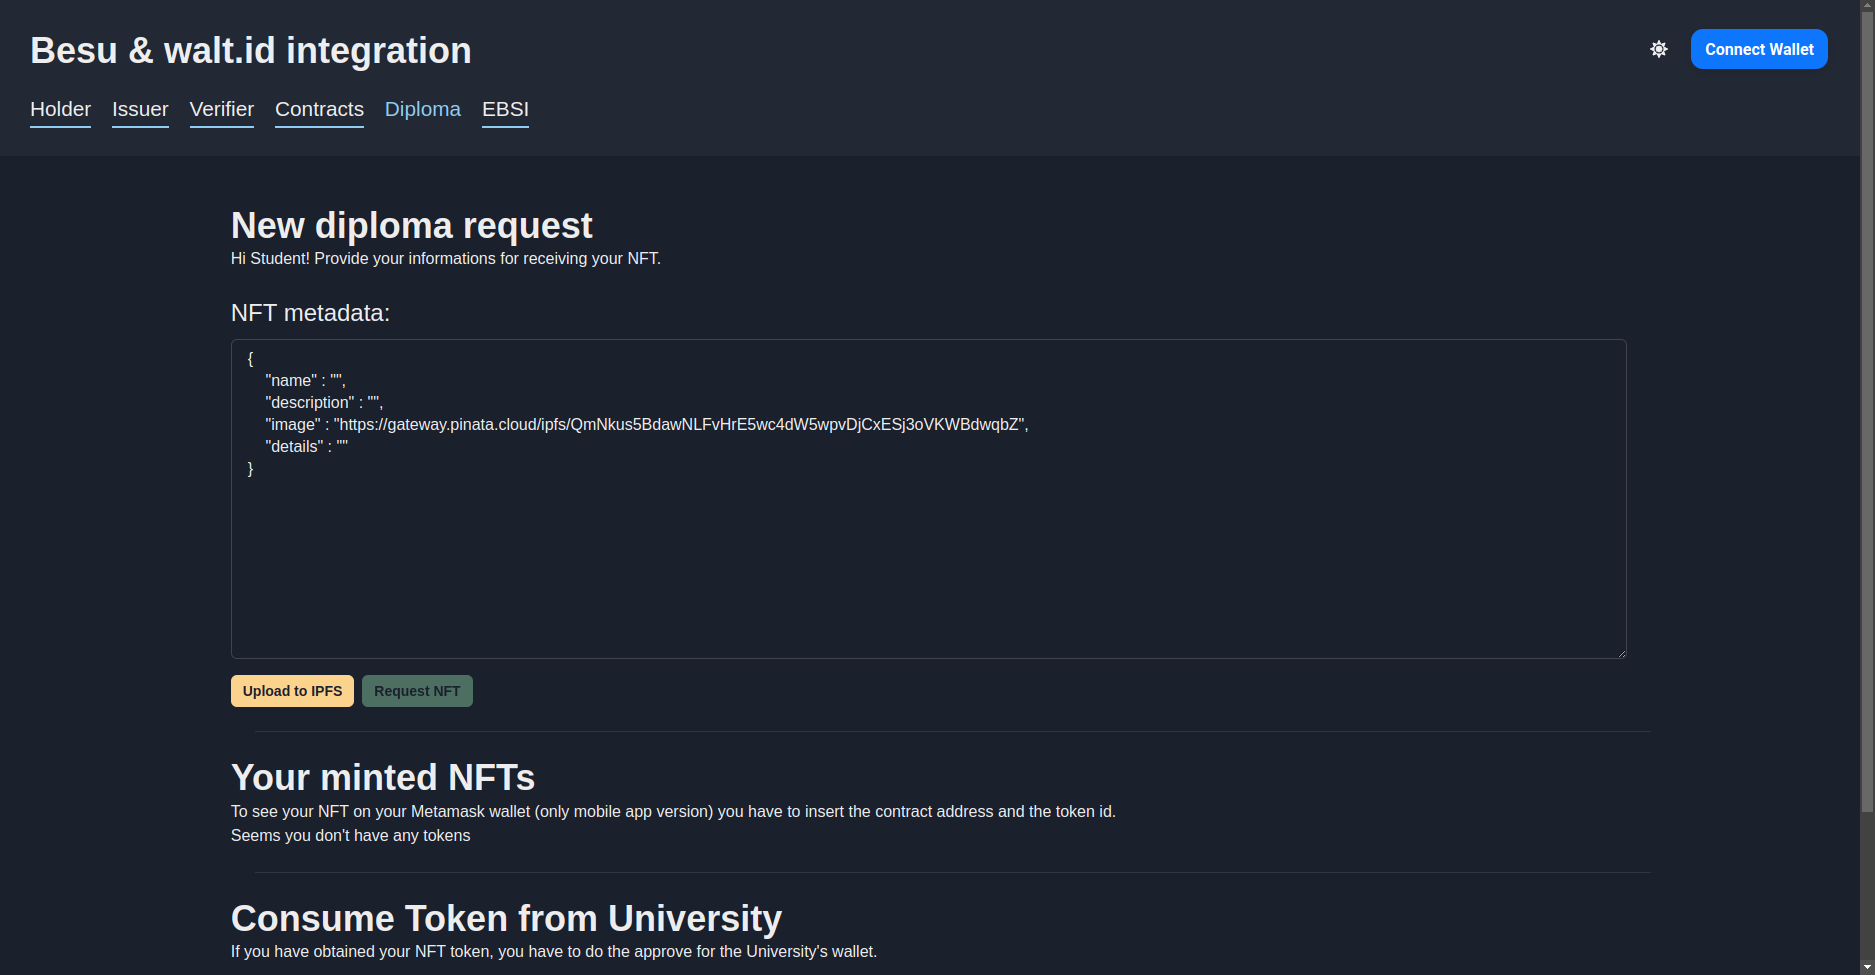
\includegraphics[width=\linewidth]{chapter3/frontend/diploma.png}
    \end{tcolorbox}
    \captionof{figure}{The \texttt{Diploma} page}
\end{center}
\clearpage
On this page\footnote{The details of this whole operation are not explained in this paper,
as they are examination subjects of another student's thesis.}:
\begin{itemize}
    \item A student can request an NFT usable by the user to officially request the diploma;
    \item The university sees all the NFT requests and can accept them by minting
    the Request NFT to the student's wallet;
    \item A student can approve the university to burn the Request NFT; after that,
    the university can consume (or burn) the Request NFT and issue the VC diploma to 
    the student (issuing procedure is not implemented).
\end{itemize}

\vspace{1cm}
\subparagraph{EBSI.} Figure 3.14 shows the page screenshot.
\begin{center}
    \begin{tcolorbox}[
        beamer,
        width=0.6\textheight,
        arc=0pt,
        boxsep=0pt,
        left=0pt,right=0pt,top=0pt,bottom=0pt,
        ]
    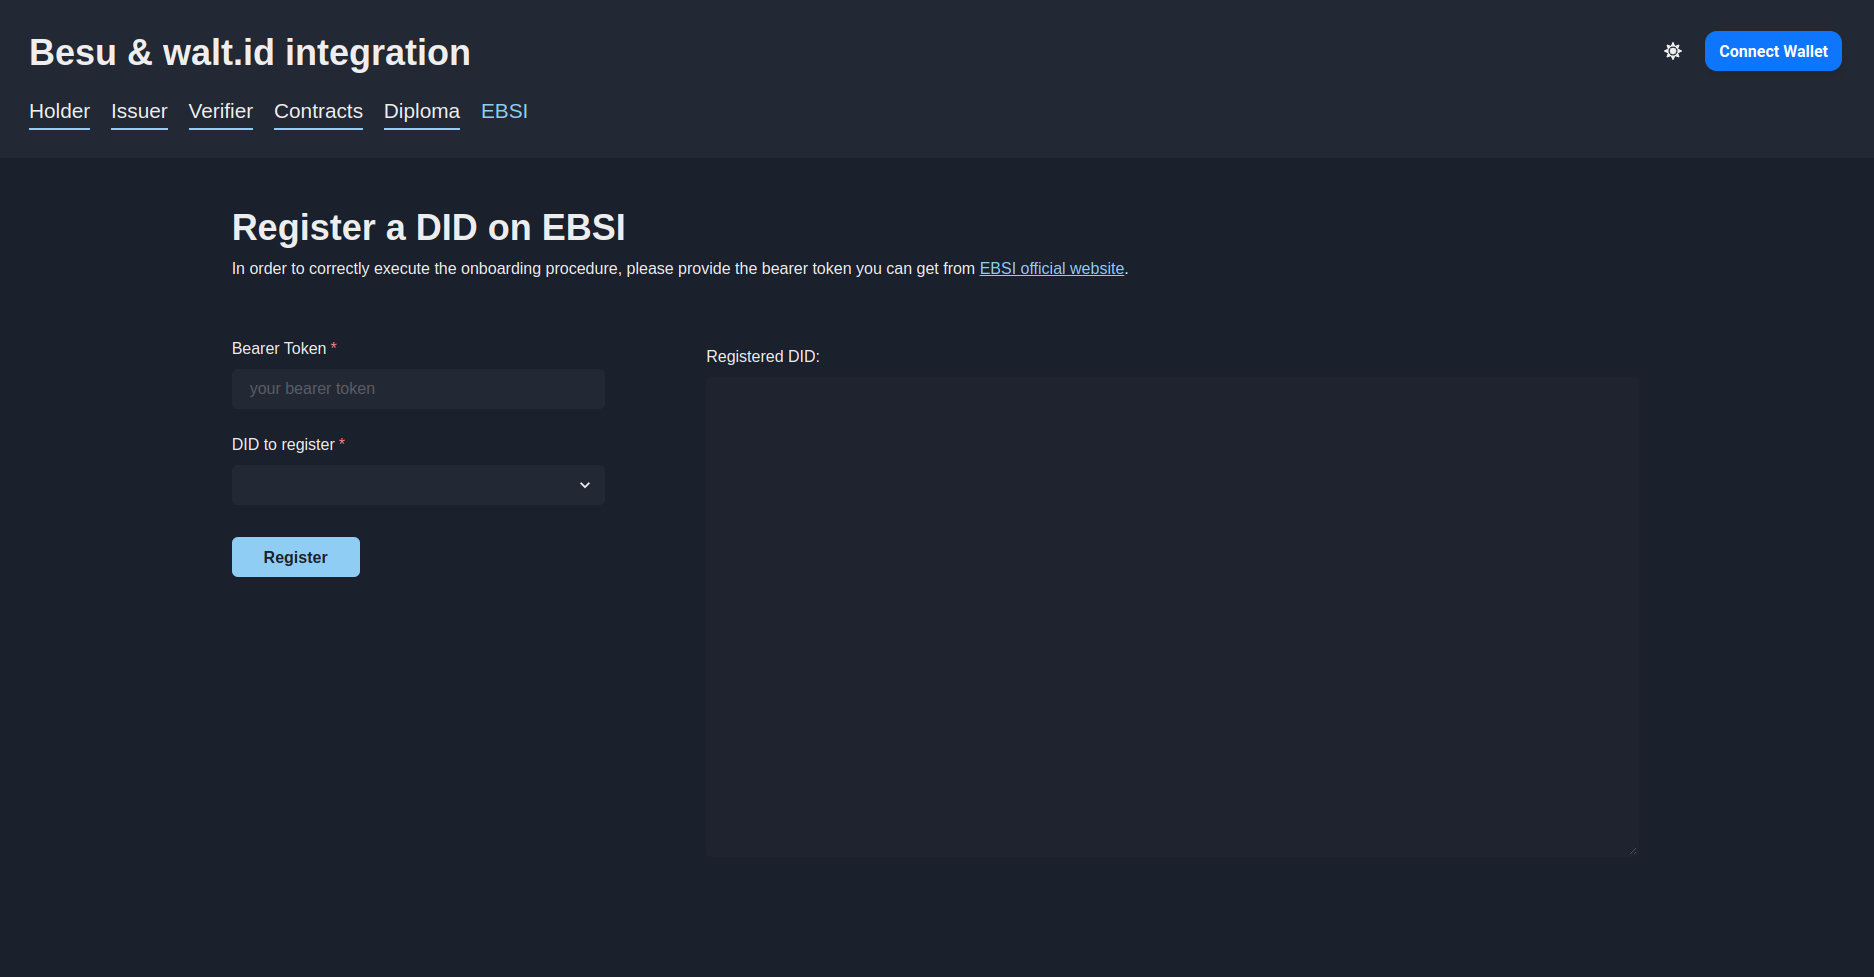
\includegraphics[width=\linewidth]{chapter3/frontend/ebsi.png}
    \end{tcolorbox}
    \captionof{figure}{The \texttt{EBSI} page}
\end{center}
\vspace{0.3cm}
A user can register a DID on the EBSI network on this page. The user must insert
the \texttt{bearerToken}, obtainable on the EBSI official website. The interface
simplifies the registration process: as explained in the SDK section,
the process needs three steps, but the user sees only one.

\clearpage
\paragraph{Backend.}
The backend is designed as a REST API. We used it to implement the creation 
and verification of the signatures made by the verifiers when they register 
on-chain a verification record.
\vspace{0.3cm}\\
The functions made available to the frontend are two:
\begin{itemize}
    \item \code{/createSignature}: the verifier signs the verification record
    with its DID private key. In the request body, the verifier must insert the
    \texttt{JSON signatureRequest object}, which has two fields: \texttt{keyId},
    where is specified the private key (public) ID, and \texttt{message},
    which is the message to sign (in this case, the verification record);
    the call response is the signature in \texttt{JWS} format;
    \item \code{/verifySignature}: any user (from the frontend, if the
    interface is implemented) can verify a signature. In the request body, the
    verifier must insert the \texttt{JSON verificationRequest object}, which has
    three fields: \texttt{verifierDid}, where specified the DID of the
    verifier who signed the message, and \texttt{message}, which is the
    message to verify (also in this case, the verification record: if the
    verification record data coincides with the decoded signature payload,
    then the signature is valid and the verification record is valid too);
    if the signature is valid, the call response is the signature payload (which
    should be equal to the verification record), otherwise the function
    will throw an error.
\end{itemize}

\subsubsection{Problems and difficulties found}
Generally, we have not found crucial problems during the PoC development. The only 
difficulty was the signature creation; it took a while to find the real 
problem (i.e., the \texttt{Secp256k1} curve incompatibility with the W3C Web 
Cryptography API). Also, we had to compromise: verifiers, to generate the signature, 
can only use DID created with the \texttt{ebsi} method (so also with \texttt{Secp256k1}
curve). The \texttt{/verifySignature} has to be revisited to enhance interoperability
with other methods and encryption algorithms.

\section{Discussion}
In this last section, we discuss the last considerations about the final result, what 
can be done to improve the solution, and some personal thoughts.

\subsection{Achievements}
We partially merged the off-chain and on-chain solutions. The verifier integration works well,
also from a security point of view, thanks to the signatures implementation.\\
Thanks to the existing standards (which are in development), we created a system where 
users can own their credentials. We created an SDK that simplifies the interaction with 
SSI primitives, a smart contract suite that reflects on-chain the off-chain events, and 
the proof of concept web application gives an idea of what a user can do with the final 
solution.
So objectively, we reached a satisfying grade of requirements fulfillment, as initially
we were not sure about the possibilities.

\subsection{Acquired knowledge}

\subsection{Future developments}
It is obvious to remark that we are only at the beginning of SSI solutions development. 
Standards are being defined now, and developers do not know the right path to pursue 
since it is an exploration.
There can be many future developments for these solutions and the SSI model, especially
for seamless integration with permissionless blockchains. Let us divide them into two 
categories: PoC improvements and SSI challenges.
\subsubsection{PoC improvements}
Some of the possible PoC improvements are:
\begin{itemize}
    \item \textbf{Revocations}: they could be forced to be instantly reflected on-chain
    with a smart contract call after the revocation is made on the off-chain side, as
    is already done for verifications;
    \item \textbf{Diploma issuance}: when a user consumes the Request NFT, the university
    should be able to see it from the frontend and issue the diploma in a guided and
    easier way provided by the \texttt{Issuer} page;
    \item \textbf{Issuer}: the \texttt{Issue} section could be significantly improved from
    a UX perspective, as it is now a basic form, easy to use just for a developer who
    knows what he is doing;
    \item \textbf{Secure communication protocols}: a thing that we did not implement is the
    secure verifiable credential exchange. Fortunately, walt.id kits provide API to
    implement this feature, so it is possible to add it in the future also using those kits;
    \item \textbf{On-chain DID signature check}: it could be helpful to move the signature 
    verification (now provided by the frontend through \code{/verifySignature}) to the 
    smart contract level when a verification record is being created;
    in this way, the transaction could be reverted if the signature is not valid (i.e., 
    the verifier is not signing with the DID private key), and no one should check if 
    the signature is valid as if it is on-chain it is valid;
    \item \textbf{Sign with new DID methods}: currently, the only DID method supported 
    for the signature creation, and so for the verifiers' functions, is \texttt{ebsi}; 
    at least should be added the \texttt{key} method, to enhance the product usability.
\end{itemize}
\subsubsection{SSI challenges}

\subsection{Personal evaluation}
